\documentclass[journal,10pt,twocolumn]{article}
\usepackage{graphicx, float}
\usepackage[margin=0.5in]{geometry}
\usepackage{amsmath, bm}
\usepackage{array}
\usepackage{booktabs}
\usepackage{xfrac}
\usepackage[utf8]{inputenc}
\providecommand{\norm}[1]{\left\lVert#1\right\rVert}
\let\vec\mathbf
\newcommand{\myvec}[1]{\ensuremath{\begin{pmatrix}#1\end{pmatrix}}}
\newcommand{\mydet}[1]{\ensuremath{\begin{vmatrix}#1\end{vmatrix}}}

\title{\textbf{circle Assignment}}
\author{Harsha sai sampath kumar}
\date{September 2022}

\begin{document}

\maketitle
\paragraph{\textit{\large Problem Statement} -If the tangent at the point P  on the circle $x^2+y^2+6x+6y=2$ meets a straight line $5x-2y+6=0$         at a point Q on the y-axis then the length of PQ is }

\section*{\large Solution}

\begin{figure}[H]
\centering
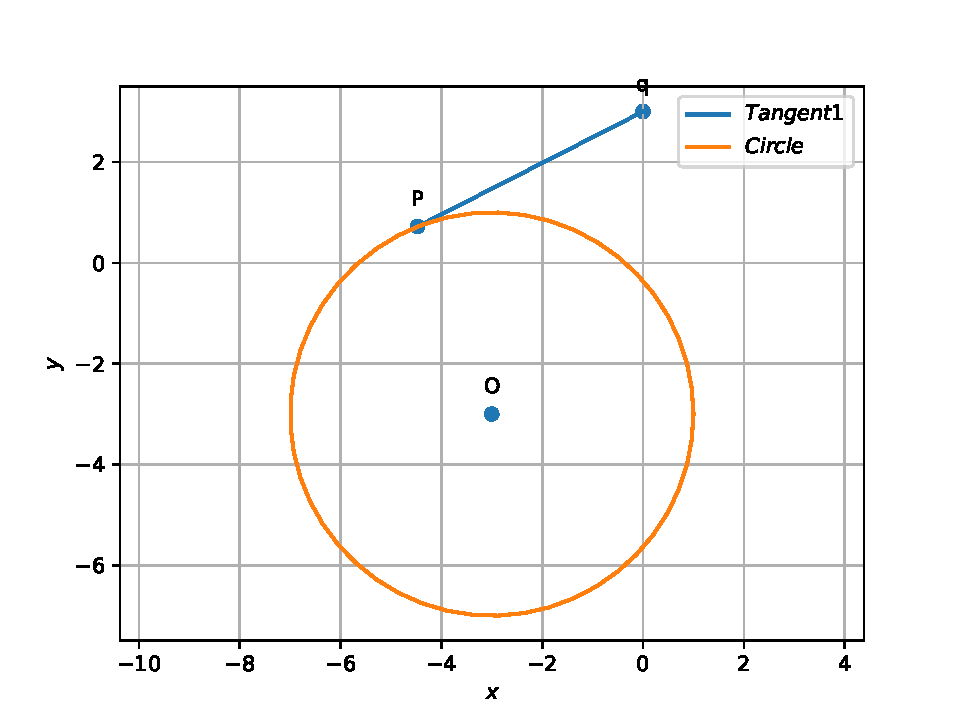
\includegraphics[width=1\columnwidth]{fig}
\caption{}
\end{figure}

\section{construction}


\begin{tabular}{|c|c|c|}
	\hline
	\textbf{Point}&\textbf{Value}&\textbf{Description}\\
	\hline
	q&(0,3)&  given point\\
	\hline
	o&(-3,-3)& centre of circle\\
	\hline
	
	
	
\end{tabular}\\







The line equation is


\begin{align}
5x-2y+6=0
\end{align}

for point Q
\begin{eqnarray}
{(5 \;-2)}
\myvec{x\\y}=-6
\end{eqnarray}


\begin{eqnarray}
\vec{n^Tx}=c
\end{eqnarray}

\begin{eqnarray}
{(5 \;-2)}
\myvec{0\\k}=-6
\end{eqnarray}

\begin{center}
-2k=-6\\
k=3
\end{center}

\begin{eqnarray}
\vec{Q}=\myvec{0\\3}
\end{eqnarray}
Given circle equation is \begin{align}
x^2+y^2+6x+6y-2=0
\end{align}
\begin{align}
\vec{x}^T\vec{Vx}+2\vec{U}^T\vec{x}+f=0
\end{align}
\begin{eqnarray}
V=\myvec{1&0\\ 0 &1} \; u=\myvec{3\\3} \;  f=-2
\end{eqnarray}

\large{If $\vec{V}^{-1}$ exists, given normal vector $\vec{n}$, the tangent points of contact to equation(2) are given by,}
\begin{align}
\vec{q_i}=\vec{V}^{-1}(k_i\vec{n}-\vec{u})^T \\
where,k_i=\pm \sqrt{\frac{f_0}{\vec{n}^T\vec{V}^{-1}\vec{n}}}\\
f_0=\vec{u}^T\vec{V}^{-1}\vec{u}-f\\
\end{align}



The normal vectors of tangents from a point $\vec{h}$ to the conic(7) are given by'
   \begin{align}
   \vec{n_1}=\vec{P}\myvec{\sqrt{\lambda_1}\\ \sqrt{\lambda_2}},\vec{n_2}=\vec{P}\myvec{\sqrt{\lambda_1}\\ -\sqrt{\lambda_2}}
   \end{align}
where $\lambda_i,\vec{P}$ are eigen parameters of 
\begin{align}
\sum=(\vec{V}\vec{h}+\vec{u})(\vec{V}\vec{h}+\vec{u})^T-\vec{V}(\vec{h}^T\vec{V}\vec{h}+2\vec{u}^Th+f)
\end{align}
   So, by solving above equation,
   \begin{align}
   \vec{n_1}=\myvec{-6.4721\\-1.7639},\vec{n_2}=\myvec{-2.472\\6.236}
   \end{align} 
   By solving equation(10), using (8),(13) and (11), we get,
   \begin{align}
   k=\pm0.596
   \end{align}
   Solving equation(9), using (8),(13) and (16), we get,
   













   \begin{align}
   \vec{p}=\myvec{-4.474\\0.718}
   \end{align}

























Distance between two points:
\begin{eqnarray}
\norm{\vec{P}-\vec{Q}}
\end{eqnarray}
 Length of $\vec{PQ}$=5




\end{document}
